\chapter{\label{ch:experimentandresult}Experiments and results}
In this chapter a comparison of wavelets discussed in chapter  \ref{ch:wavelets} is analyzed with characteristic scenes in 2D(flatland) and 3D. Such a comparison can never be exhaustive due to the heterogeneous nature of input scenes. Therefor scenes with different kind of kernels has been chosen for comparison of performance of the wavelets. We first discuss kernels for which we have the exact analytical solution of the integral equation. Then we test and compare the wavelets the 2D scenes knows as flatland scenes. Flatland scenes are selected mainly to analysis and understanding different aspects of wavelet basis for radiosity. Results of using the different wavelets with 3D scenes are also discussed at the end this chapter. \\

{\bf Ground truth comparison}\\
\section{IE with degenerate kernel}
For comparing the approximate solution with exact ground truth we chose kernels which are classified as degenerate kernels. Degenerate kernels are kernels which can be expanded in the form shown in Equation (\ref{eq:kxydegenexpansion})
\begin{equation} \label{eq:kxydegen}
K(x,y) = \sum\limits_{i=1}^na_i(x)b_i(y) \\ 
\end{equation}
An integral equation with degenerate kernel can be solved by changing the order of integral and summation after substituting expanded kernel. See a
Appendix \ref{apen:derivationdegenerate} for analytical solution of non-homogeneous Fredholm IE of second kind. 

We took kernel $K(x,y)=(x-y)^2$ and $K(x,y)=x^4+y^2$ for comparing different wavelets with the ground truth solution $B(x)=${\bf find the solution} of the IE shown in Equation \ref{eq:genrie}

We compare wavelets by calculating error in the projection of kernel $K(x,y)$ and error in solution $B(x)$. The metric used for comparison is relative error as shown in Equation \ref{eq:Krelerr}. It is a ratio of $L^2$ norm of error $(K(x,y)-\hat{K}(x,y))$ to $L^2$ norm of kernel. The integration is over entire domain of x and y. Where $\hat{K}(x,y)$ is approximation of $K(x,y)$ in space spanned by chosen wavelet.
\begin{equation} \label{eq:Krelerr}
\text{relative  error}=\frac{\int\int \,(\,K(x,y)-\hat{K}(x,y)\,)^2  \,dy \, dx}{\int\int \,K(x,y)^2  \,dy \, dx}
\end{equation}
The purpose of selecting degenerate kernel is to make sure that the implemented algorithm works properly and algorithm is fit for testing the wavelets with the scenes for which we do not have the ground truth analytical solution. Note that the kernels discussed in this section does not describe any real world scene. We first take the kernel $K(x,y)=(x+y)^2$ which can be expanded as shown in Equation \ref{eq:kernelanalytical1}. This kernel is of the form shown in Equation \ref{eq:kxydegenexpansion}. The domain of variable is [0,1]




\begin{equation} \label{eq:kernelanalytical1}
K(x,y)=(x+y)^2=x^2+2xy+y^2 \quad x,y \in [0,1]
\end{equation}



We substitute this kernel in Equation \ref{eq:genrie} to get,
\begin{eqnarray} \label{eq:analytical1}
B(x)=E(x)+\int\limits_0^1 K(x,y)B(y) dy \\
 = E(x)+\int\limits_0^1 (x+y)^2 B(y) dy
\end{eqnarray}

solution for above IE,

\begin{equation} \label{eq:solutinoanalytical1}
B(x)=
\end{equation}
The solution, $B(x)$, in above Equation \ref{eq:solutinoanalytical1} is calculate analytically using the method shown in Appendix \ref{apen:derivationdegenerate}. This ground truth solution is used to compare approximate solution of different wavelets. Approximate solution is calculate using projection method shown in Chapter \ref{ch:waveletprojection}. Figure \ref{fig:replacethis} shows the approximate solution and error function with different wavelets without thresholding(replacing negligible elements  with value 0) \underline {show equation of error and projected solution in chapter \ref{ch:waveletprojection} or else show it here}. As we can see that as the vanishing moment of wavelet increases the error decreases. \underline{ This is because higher order wavelets can approximate the kernel and solution more accurately. Figure \ref{fig:replacethis1}  shows that if we increase n error reduces. Above two result shows that to decrease error in  solution either n or order basis function has to be increased Aslo for QLMW error is zero for all n because $K(x,y)$ lies in space spanned by QLMW basis}



\begin{figure}[tbh]
\centering{}
\captionsetup{justification=centering}
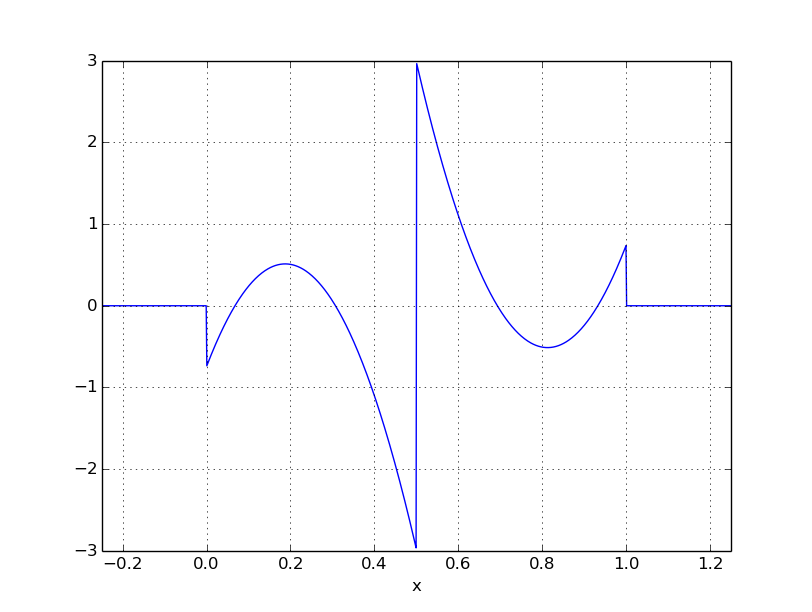
\includegraphics[width=3in]{qlmwpsi2.png}
\caption{\label{fig:replacethis}Haar wavelet llmw qlmw CAS solution error and error l2 value n=4 and n=16}
\end{figure}

\begin{figure}[tbh]
\centering{}
\captionsetup{justification=centering}
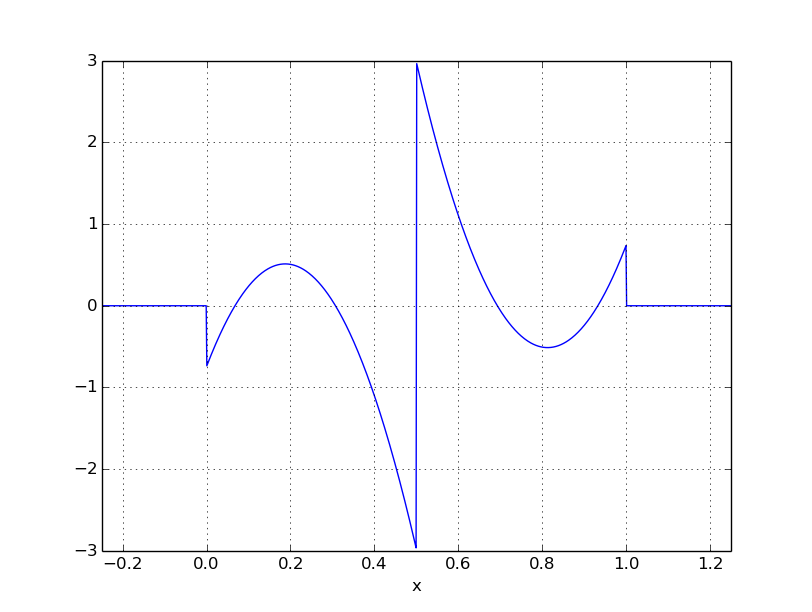
\includegraphics[width=3in]{qlmwpsi2.png}
\caption{\label{fig:replacethis1}Haar wavelet llmw qlmw CAS error plot with increasing n}
\end{figure}


\section{Flatland radiosity}
In this section we discuss the comparison of different wavelets to solve radiosity for flatland scenes. Flatland is two dimensional world in which surfaces are one dimensional instead of two dimensional surfaces in three dimensional scene. We select flatland scenes for its simplicity and imaginability of kernel associated with scenes. Simplest flatland scene is scene with two parallel line segment of unit length each(see Figure \ref{fig:replacethis2}) and scene with two line segment, of unit length each, perpendicular to each other(see Figure \ref{fig:replacethis3}). 



\begin{figure}[tbh]
\centering{}
\captionsetup{justification=centering}
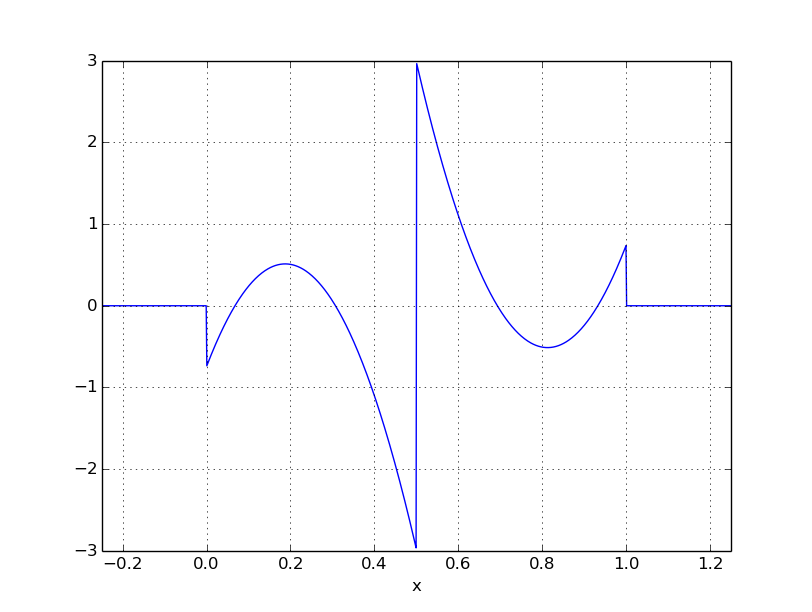
\includegraphics[width=3in]{qlmwpsi2.png}
\caption{\label{fig:replacethis2}flatland1 scene: parallel line segment x axis and y axis different of unit length}
\end{figure}


\begin{figure}[tbh]
\centering{}
\captionsetup{justification=centering}
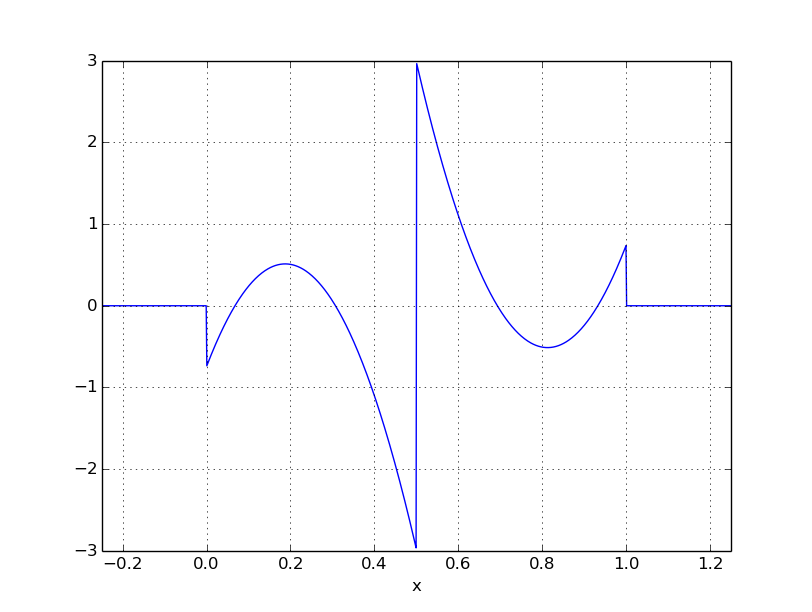
\includegraphics[width=3in]{qlmwpsi2.png}
\caption{\label{fig:replacethis3}flatland2 scene: perpendicular line segment x axis and y axis different of unit length each}
\end{figure}

Note that $x \in X$ and $y \in Y$ in above kernels. $K(x_1,x_2) = 0$ for $x_1,x_2 \in X$ as two points in a line segment do not interact directly, however they can interact indirectly through reflections from other line segment(see Figure \ref{fig:replacethis4}) for graphical representation of kernel of any two line segment in general. In other words interaction can take place only between two different planner surfaces(on lines in this context) on however, two points on single concave surface(or line) can interact directly.  The kernel $K(x,y)$ of flatland is calculated using \underline{give reference}. We will refer to scene consist of parallel line segment as flatland1 and scene with two perpendicular line segment as flatland2. Kernel $K_1{x,y}$ for flatland1 is


\begin{figure}[tbh]
\centering{}
\captionsetup{justification=centering}
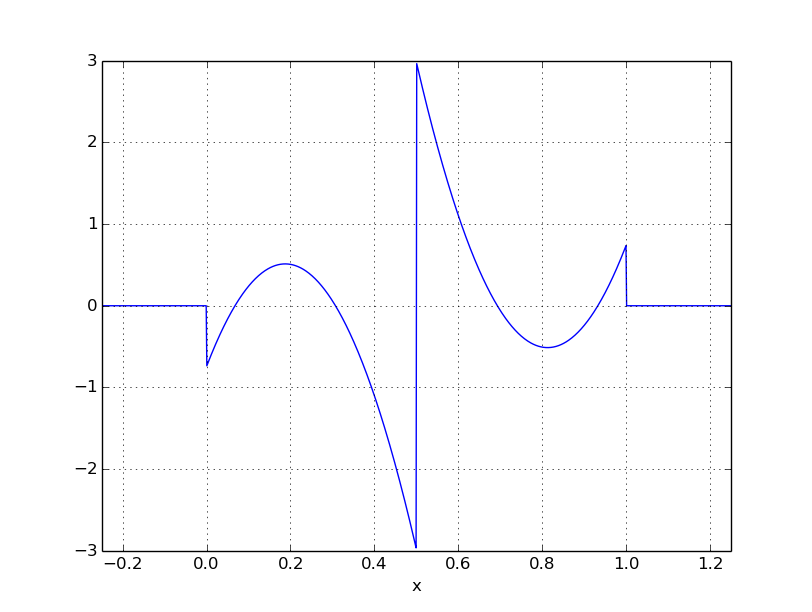
\includegraphics[width=3in]{qlmwpsi2.png}
\caption{\label{fig:replacethis4}flatland scene kernel in general with zero and non zero regions}
\end{figure}


\begin{eqnarray} \label{eq:kernelflatland1}
K_1(x,y)\quad=\frac{   \cos{\theta_x}  \cos{\theta_y}  }{    2\,r_{x,y}   }\quad\quad\quad\\
        =\frac{dist^2}{2((x-y)^2+dist^2)}
\end{eqnarray}
and kernel  $K_2{x,y}$ for flatland2 is

\begin{eqnarray} \label{eq:kernelflatland2}
K_2(x,y)=\frac{\cos{\theta_x}\cos{\theta_y}}{2\,r_{x,y}} \quad\quad\quad\\
=\frac{xy}{2(x^2+y^2)^{\frac{3}{2}}}\quad\quad\quad
\end{eqnarray}
We can change distance between two line segment in flatland1 to get different scene. As the distance decrease interaction between two segment increases. Figure \ref{fig:haarscalesparsef1} and \ref{fig:haarwaveletsparsef1} shows the kernel of flatland1 with $dist=0.25$. The kernel is non negative over entire domain. Also the interaction between two points is maximum when distance between them is less. Kernel is projected into space spanned by wavelet basis to get the sparse matrix of coefficient as shown in \ref{fig:replacethis6} \ref{fig:replacethis7} \ref{fig:replacethis8}\ref{fig:replacethis9} \ref{fig:replacethis10} \ref{fig:replacethis11}. \underline{also refer to CAS and thik about putting this images here instead of wavelet projection chapter} \\

To plot the sparsity of matrix we plot sorted elements of matrix. Figure \ref{fig:sortedhaar}
{\bf show all the distance and and f2 comment on increase in element value vs decrease in distance also show poly-poly and wavelet-poly copmparison for conclusion purpose }

\begin{figure}[tbh]
\centering{}
\captionsetup{justification=centering}
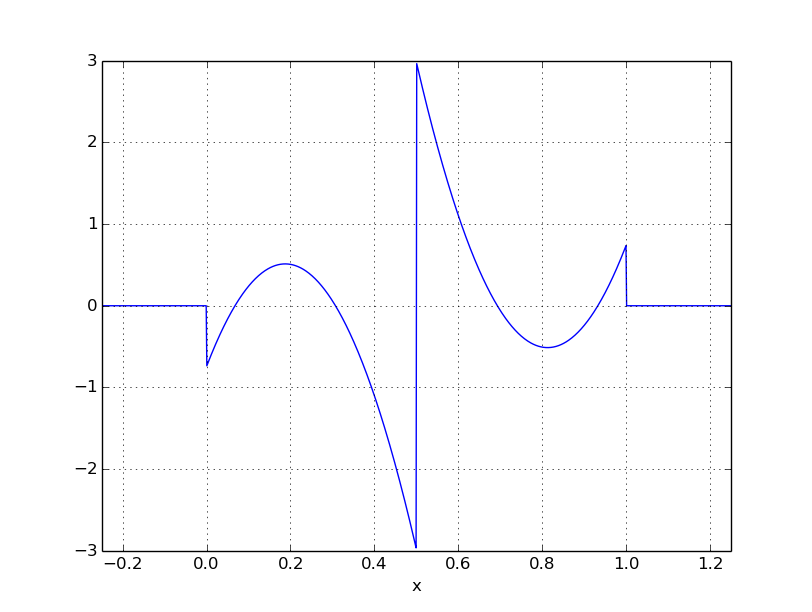
\includegraphics[width=3in]{qlmwpsi2.png}
\caption{\label{fig:replacethis5}flatland1 with $dist=0.25$ kernel mesh plot}
\end{figure}
\begin{figure}[tbh]
\centering{}
\captionsetup{justification=centering}
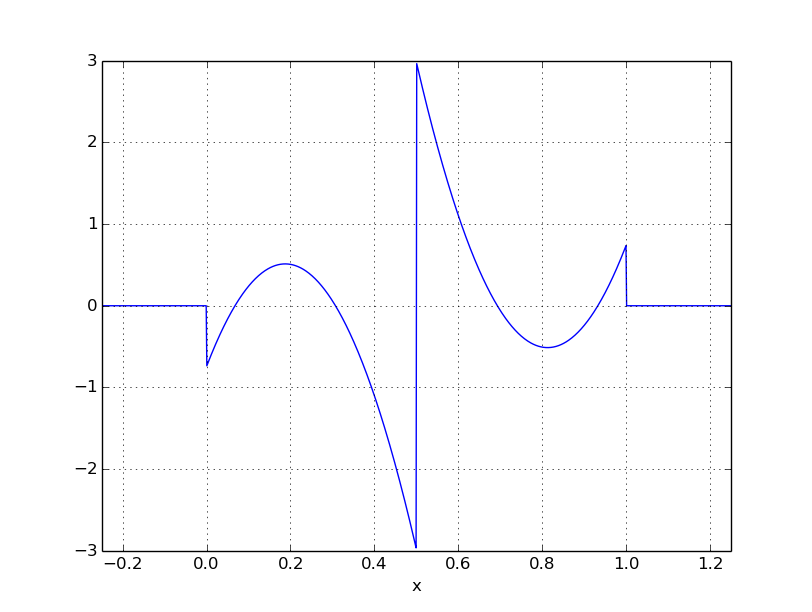
\includegraphics[width=3in]{qlmwpsi2.png}
\caption{\label{fig:f10.25sortedhaar}flatland1 with $dist=0.25$ sorted elements}
\end{figure}

Figure \underline{show figure of error vs top n haar wavelet poly f10.25} the relaton between error in projection and top n element in terms of values while other elemets are replaced with zero value (thresholding) in radiosity matrix projected using haar wavelet and haar scalling function. Let the this process of replacing small values with zero be refered as {\em thresholding} As we can see, wavelet basis gives us more sparsity after thresholding error in pojection is less as compared to scaling function basis. Figure \underline{show for other wavelets} shows similar reults with LLMW and QLMW. Figure \underline{show result for all the scenes mension details in caption} shows result for different scenes which shows the similar results.
% \begin{eqnarray} \label{eq:kernelflatland1}
% 

% \end{eqnarray}

% \begin{eqnarray} \label{eq:kernelflatland1}
% K_1(x,y)=\frac{\cos{\theta_x}\cos{\theta_y}}{2\,r_{x,y}}\\
% =\frac{dist^2}{2((x-y)^2+dist^2)}

% \end{eqnarray}

% and kernel  $K_2{x,y}$ for flatland2 is


% \begin{eqnarray} \label{eq:kernelflatland2}
% K_1(x,y)=\frac{\cos{\theta_x}\cos{\theta_y}}{2\,r_{x,y}} \quad x,y \in [0,1]
% \end{eqnarray}








\section{Three Dimensional Rasioity}
In this section we show reults of projection method to solve 3D radiosity. Scene which we chose is shown in Figure \underline{show parallel  scene}. we divided each surface into grid of  \underline{n*n}  elements of equal size and assumed the radiosity function, over the domain of surface, to be piecewise constant over each element. Thus we have projected radiosity function into space spanned by dilates and translates of two dimensional Haar scaling function. We use projection method discussed in Chapter \ref{ch:waveletprojection}. To get system of linear equations which are solved to find the unknown projected function. Figure \underline{show result of haar wavelet in red color } shows the solution and images of the scene. Similar to Haar wavelet we can use LLMW and QLMW for projection methods. In case of LLMW we are dealing with space of piecewise linear functions and LLMW wavelet forms the basis for the same space. In case of QLMW, we are dealing with space of piecewise quadratic function for which QLMW wavelet serves as alternative basis. Use of this alternative basis give us advantage of sparse matrix for which matrix inversion is faster. Figure    \underline{show result of LLMW and QLMW wavelet in red color also show the spots of the function} shows the solution and images of the scene







.\\\\\\\\\\\\{\bf flatland}\\

{\bf 4d}\\
\\section{Radiosity in three dimension} % (fold)
\label{sec:radiosity_in_three_dimension}
\underline{solution and threshold solution}
% section radiosity_in_three_dimension (end)
